\documentclass{article}
\usepackage{import}
\subimport{../}{preamble}
\begin{document}

\section{Understanding Plasmons in Spherical Nanoparticle Tips}

\begin{figure}[bt]
\centering
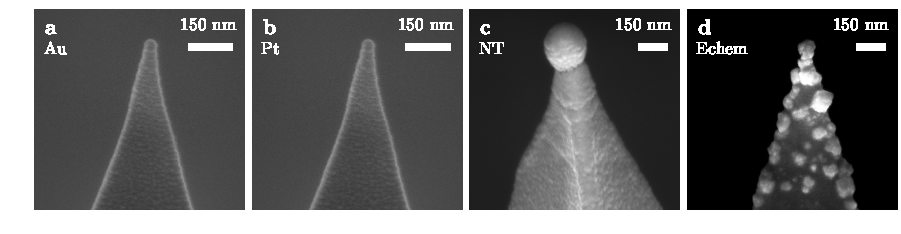
\includegraphics{figures/tip_sems}
\caption[SEM images of sharp and spherical metal tips studied using hyperspectral imaging]{\textbf{SEM images of sharp and spherical metal tips studied using hyperspectral imaging.} Tips are  (a) a sharp Au AFM tip, (b) a sharp Pt AFM tip, (c) a NT Au-coated spherical AFM tip and (d) an electrochemically deposited AuNP-on-Pt AFM tip.}
\label{fig:tip_sems}
\vspace{-10pt}
\end{figure}

% Lead into hyperspectral images and tip comparisons
Hyperspectral images are taken of four different types of AFM probes to investigate the plasmonics of nanostuctured tips. AFM tips studied are Au- and Pt-coated standard AFM probes (BudgetSensors Au-coated AFM probes), spherical Au tips (\SI{300}{nm} Au-coated NanoTools B150 AFM probes) \cite{savage2012} and AuNP-on-Pt AFM probes, fabricated in-house using electrochemical deposition \cite{sanders2014}. SEM images of a selection of these tips are shown in \autoref{fig:tip_sems}. Fabricated tips are pre-treated where possible prior to use with piranha solution to remove organic surface residue and, in some cases, smooth surface roughness. % is the cleaning necessary since this isn't a sub-nm contact paper?

\begin{figure}[bt]
\centering
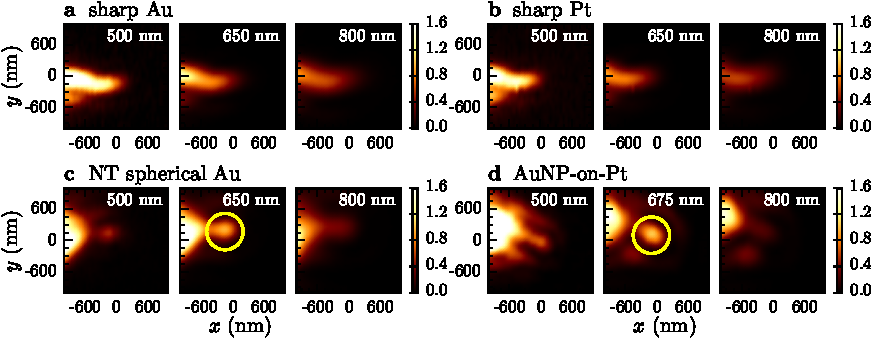
\includegraphics{figures/hyperspectral_tip_comparison}
\caption[Hyperspectral images of sharp and spherical metal tips at wavelengths of interest]{\textbf{Hyperspectral images of sharp and spherical metal tips at wavelengths of interest.} Images are of (a) a sharp Au tip, (b) a sharp Pt tip, (c) a NanoTools Au-coated spherical tip and (d) an electrochemically deposited AuNP-on-Pt tip. Collection polarisation is along the tip axis. Colour maps between slices all have the same normalisation. Resonant scattering from spherical apices is clearly seen in the hyperspectral images of between 600-\SI{700}{nm} and highlighted by yellow circles.}
\label{fig:hyperspectral_tip_comparison}
\vspace{-5pt}
\end{figure}

% Brief description of hyperspectral results
Comparisons between spherical- and sharp-tipped metallic probes using hyperspectral image slices (\figurename~\ref{fig:hyperspectral_tip_comparison}) show that spherical Au tips exhibit a characteristic red (600--\SI{700}{nm}) scatter, delocalised from the bulk tip. No similar localised scattering is seen for sharp Au or Pt tips in the visible spectrum, which have an overall weaker optical response. This delocalised apex scatter can also be clearly seen in wide-field DF imaging. SEM images confirm that this scatter correlates only with spherical Au tip shapes, or when a AuNP is securely attached at the tip apex with a sufficiently small neck joint.

% Show apex spectra comparison here
\begin{figure}[bt]
\centering
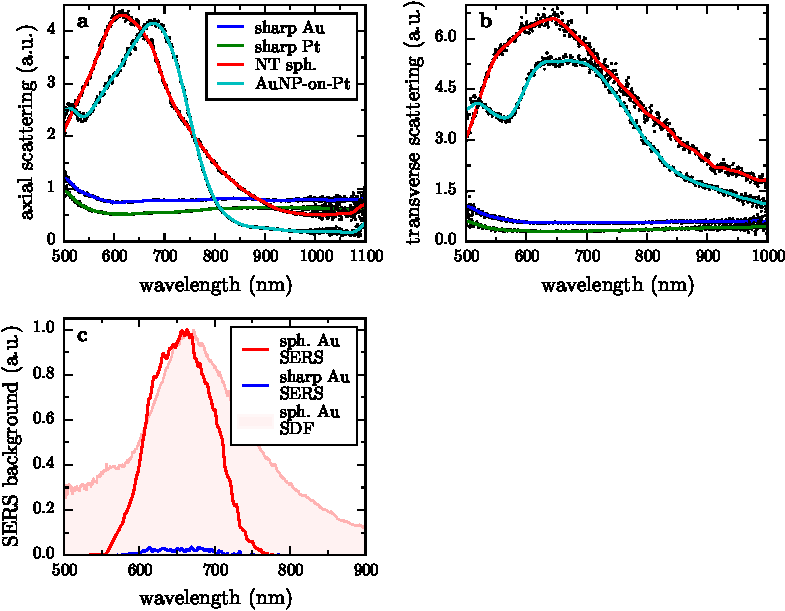
\includegraphics{figures/apex_spectra_comparison}
\caption[Apex spectra of sharp and spherical metal tips]{\textbf{Apex spectra of sharp and spherical metal tips.} Spectra are extracted from the hyperspectral images in Fig.~\ref{fig:hyperspectral_tip_comparison} by integrating pixels around the apex region. A clear resonance at \SI{630}{nm} is observed with spherical tips in both polarisations. The axial/longitudinal tip resonance is blueshifted \SI{20}{nm} from the longer transverse resonance. Sharp metallic tips show comparatively flat spectra.}
\label{fig:apex_spectra}
\vspace{-5pt}
\end{figure}

% Apex spectra comparisons
Integrating spectra around tip apices confirm that only spherical Au tips exhibit structural resonances (\figurename~\ref{fig:apex_spectra}). Scattering resonances around \SI{630}{nm} are reliably present in all spherical-tipped AFM probes, both vacuum-processed and electrochemically deposited AuNP-on-Pt, and are attributed to direct LSP excitation. The response of sharp Au tips shows no similar plasmonic features while the slow rise in scattering towards the NIR is consistent with lightning rod scattering \cite{zhang2009}.

% Validation of SDF spectra and plasmonic observations
\begin{figure}[bt]
\centering
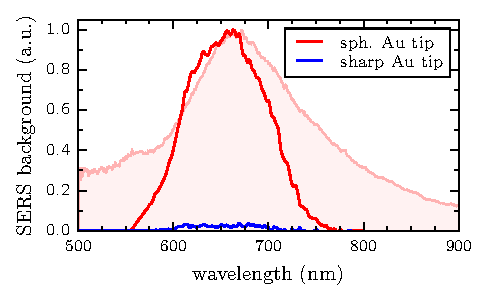
\includegraphics{figures/lsp_confirmation}
\caption[Integrated inelastic electron fluorescence measurements of both a sharp and spherical Au tip]{\textbf{Integrated inelastic electron fluorescence measurements of both a sharp and spherical Au tip.} Fluorescence spectra are acquired using tuneable, single wavelength spectroscopy with integrated spectra plotted as a function of excitation wavelength. The background spectrum is the supercontinuum dark-field scattering spectrum of the spherical Au tip apex, as measured using hyperspectral imaging. Agreement between the fluorescence (near-field) and dark-field scattering (far-field) spectra confirms resonant near-field enhancement as a \gls{lsp} excitation. Sharp Au tips show no such resonance in either the near-field or far-field.}
\label{fig:lsp_confirmation}
\vspace{-5pt}
\end{figure}

Broadband tuneable SERS \cite{lombardi2015} on each of the tips is used to confirm that the resonance is indeed a LSP by showing that the internal near-field is resonantly enhanced.%
\footnote{Acquisition of broadband tuneable SERS measurements carried out by A.\ Lombardi.}
During plasmon excitation both internal and external fields are enhanced. The external field leads to the strong enhancement of Raman spectra whereas inelastic electron scatter insider the surface of the metal is enhanced by the internal field, forming the SERS background \cite{hugall2015}. Broadband tuneable SERS is a technique capable of showing both these components \cite{lombardi2015}. Hence, by integrating the inelastic scattering background at each wavelength the near-field resonance can be calculated.%
\footnote{Model of this behaviour is derived in the appendix.}
SERS background spectra are taken in \SI{10}{nm} increments of the excitation wavelength.%
\footnote{Each acquired background spectrum is shown in the appendix}
Integration of the scattering counts for each excitation wavelength shows a distinct peak (\autoref{fig:lsp_confirmation}) around the scattering resonance from \autoref{fig:apex_spectra}, confirming it as a LSP resonance. Further, confirmation stems from direct observation of plasmon coupling between spherical tips, as has been previously reported \cite{savage2012}, with results of the latest tip coupling experiments discussed in detail in the next chapter.

% Differences between types of spherical tips
Surprisingly, the overall disorder and parasitic edge AuNP nucleation on AuNP-on-Pt only minimally effects the overall optical response from the apex growth. This is likely because the spherical apex already interacts with the base tip structure, regardless of any further deposits. The AuNP-on-Pt structure behaves very similarly to the Au-coated diamond-like-carbon spherical tip, likely because the \SI{50}{nm} coating thickness is greater than the skin depth \cite{stockman2011, huber2014}. Plasmons therefore see both as solid Au spheres. Differences arise due to the differences in neck material with Au-Pt and Au-Au neck boundaries.

\FloatBarrier
\subsection{Interpreting the Spectral Response of Metallic Tips}

The plasmon modes of a spherical Au tip are not so different from those of a spherical AuNP and can be explained accordingly. Like AuNP plasmons, spherical tip LSPs are specifically \emph{radiative} antenna-like modes, those that can efficiently couple far-field light into strong collective free electron oscillations without the need for momentum matching due to SPP dispersion. As with AuNPs, the signature of these plasmons is a distinct SPR indicating their large dipole moment, as seen in \figurenames~\ref{fig:apex_spectra} and \ref{fig:lsp_confirmation}. Radiative antenna-like LSPs form only when two close dielectric surfaces surround a metallic particle, allowing the formation of confined multipolar charge oscillations where the geometry modifies the oscillation restoring forces and determines the resonant wavelength \cite{mock2002, kuwata2003}. Spherical metal tips retain some of the back hemisphere around the connection to the base tip apex (the neck), allowing the spherical apex surfaces to sustain similar antenna-like plasmons. Sharp tips do not have this back surface, hence cannot support such resonances.
Their metal-dielectric surface still, however, supports the launching of SPPs in the near-field if the correct launching conditions are satisfied. This requirement means that while a sharp tip can in some ways be considered an optical antenna its supported modes are considered as \emph{evanescent} or \emph{near-field} modes rather than \emph{radiative}, limiting its usability.

\begin{figure}[bt]
\centering
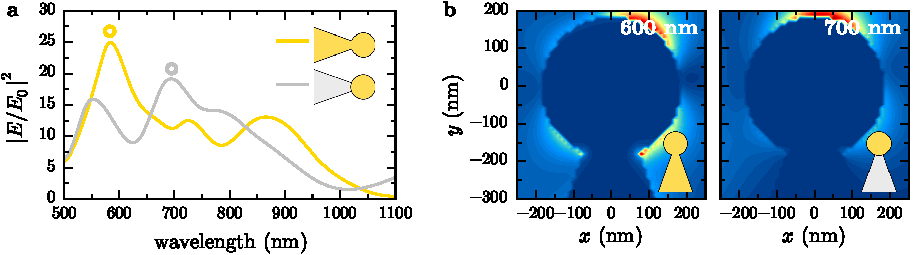
\includegraphics{figures/spherical_tip_simulations}
\caption[Numerical simulations of the field enhancement around a spherical Au tip]{\textbf{Numerical simulations of the field enhancement around a spherical Au tip.} (a) Near-field spectra of spherical Au and AuNP-on-Pt tips, extracted from around the apex of the tip. (b) Near-field enhancement distributions of the two resonances highlighted by circles in (a). Simulated tips have a \SI{300}{nm} spherical radii, \SI{120}{nm} neck widths, \SI{20}{\degree} opening angles and \SI{1.88}{\micro\metre} lengths.}
\label{fig:spherical_tip_simulations}
\end{figure}

% Near-field simulations and identification of mode charge distributions
Numerical simulations of the near-field around spherical tips, computed using BEMAX, are used to show aspects of antenna-like behaviour and can be used to qualitatively describe tips.%
\footnote{BEMAX simulations carried out by D.\,O.\ Sigle.}
Simulated spectra of the near-field around the apices of \SI{300}{nm} spherical Au and AuNP-on-Pt tips with \SI{120}{nm} neck diameters and \SI{20}{\degree} opening angles are shown in \autoref{fig:spherical_tip_simulations}a. Tips are simulated with a length of \SI{1.88}{\micro\metre} to avoid significant truncation artefacts. A neck width of $d_{\mathrm{neck}}=0.4d_{\mathrm{sphere}}$ (\SI{120}{nm} in this case) is used to match typical experimental structures. Strong modes appear for both tips between 550--\SI{700}{nm} similar to experiments. The peak positions of the strongest resonance in each tip approximately agree with the experimental spectra shown in \autoref{fig:apex_spectra}a. Near-field maps corresponding to the main resonance in each tip are shown in \autoref{fig:spherical_tip_simulations}b. The near-field at the dominant resonance in the spherical Au tip appears more quadrupole-like with a weaker dipole-like resonance occurring above \SI{700}{nm}. These are similar to the modes in the AuNP-on-Pt tip except redshifted with different intensities. The \SI{700}{nm} resonance in the AuNP-on-Pt tip has a more dipole-like structure with a more quadrupole-like resonance at \SI{550}{nm}.

Spectra can be explained by realising that quadrupolar visible modes are more favourable in larger AuNPs, as found in Mie scattering theory, once dipolar resonances shift out into the NIR. A similarly structured mode to the AuNP quadrupole plasmon would be expected in \SI{300}{nm} spherical Au tips between 500--\SI{600}{nm}. The neck geometry can potentially short the pole of dipolar plasmons, reducing their confinement, whereas quadrupolar plasmons are much less affected, leading to a more favourable charge distribution and larger SPR. Restoring forces are very different in spherical tips than nanospheres, however, since the neck removes a portion of the back sphere surface and introduces conductive losses, and the tip exiting close to the rear surface provides a secondary surface for self-interaction. This makes them difficult to analytically describe.

Electromagnetic coupling between Au and Pt surfaces is weaker than the interaction between two Au surfaces \cite{ren2004}, hence plasmons in the Au sphere are less redshifted when attached to a Pt tip apex. The non-plasmonic Pt neck region also forms an additional boundary interface to better confine plasmons to the AuNP. Hence, the redshift of AuNP-on-Pt tips is much less pronounced. The dipole-like mode exists nearer to the visible and therefore becomes more favourable than the quadrupole-like mode or becomes easier to couple to. Failure to experimentally observe the predicted quadrupole-like mode suggests that either the dipolar mode is a far more energetically favourable charge configuration or that the simulated geometry remains too dissimilar to realistic spherical tips. Nevertheless, simulations provide some insight and qualitative descriptions from which to understand plasmons in spherical metallic tips.

\begin{figure}[bt]
\centering
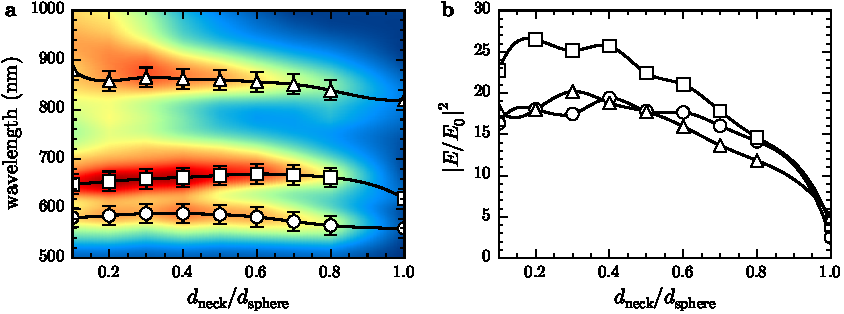
\includegraphics{figures/neck_size_dependence}
\caption[Resonant wavelength and field enhancement dependence on the neck width]{\textbf{Resonant wavelength and field enhancement dependence on the neck width.} The resonant wavelength (a) and field enhancement (b) for each of the resonances in spherical Au tips of \SI{250}{nm} sphere diameter, \SI{1.88}{\micro\metre} length, and \SI{10}{\degree} opening angle of varying neck widths.}
\label{fig:neck_size_dependence}
\end{figure}

In order to directly compare the \emph{plasmonic} behaviour of spherical Au tips with sharp Au tips independent of the lightning rod contribution, the neck width is increased in simulations with spectra extracted as before. In this manner, the structure transitions from a AuNP attached to the apex of a sharp tip into a more typical spherical tip followed by a transition into a rounded tip geometry, similar in shape to a sharp Au tip, without the radius of the tip apex ever changing.
{\color{red}A smaller radius of curvature and opening angle are used to fall between the expected behaviour of both sharp and spherical tips.}
The field enhancement and peak positions extracted from the results of this morphology transition are shown in \autoref{fig:neck_size_dependence}. Resonances do not appear to be particularly sensitive to neck width until it becomes greater than $0.8d_{\mathrm{sphere}}$ and the tip transitions into a geometry more similar to sharp tips. This explains the robustness of observed spherical tip plasmons regardless of tip morphology. A steady decrease in the field enhancement, however, is observed once $d_{\mathrm{neck}}>0.4d_{\mathrm{sphere}}$, decreasing faster once $d_{\mathrm{neck}}>0.8d_{\mathrm{sphere}}$. This supports the claim that sharp tips lack a back surface on which to sustain antenna-like LSPs.

\subsection{Implications of Spherical Metallic Tip Plasmonics}

The previously presented results demonstrate that it is important to consider what plasmons might exist in a particular nanostructure geometry under certain illumination and collection conditions, and that it is vital to characterise nanostructures before applying them in any further techniques. Without prior knowledge as to where in the visible spectrum specific plasmons are excited it is difficult to properly interpret any further results, such as TERS spectra. Improved tip characterisation is crucial to understanding why such varied TERS enhancements are reported. Additional thought must also be given to the optical method of characterisation. Confocal hyperspectral imaging is capable of mapping the local scattering response due to use of a pinhole for localisation. Broadband tuneable SERS also offers a unique way of characterising the near-field. Basic microscopy alone is a not particularly effective method for measuring the apex response of a tip and thus techniques similar to those described in this chapter should be used and developed wherever and whenever possible.

Utilising spherical tips not only exploits visible LSPs but also permits the use of a wider range of illumination configurations as the restriction to evanescent coupling is lifted. Regardless of plasmonics, the lightning rod effect will always play a role in the near-field enhancement process, giving sharp tips an initial advantage, but with careful optimisation of the spherical tip geometry, tips can be brought into resonance with one of the plasmons to maximise enhancement. Spherical Au tips in their current form are already quite well optimised for TERS due to being on resonance with the readily available HeNe laser wavelength often used.

Plasmons in spherical tips have also been shown to readily couple with plasmons in other spherical tips \cite{savage2012} and would be expected to couple with image charges in a planar mirror, thus significantly increasing their near-field enhancement. In this situation, their resonances can be tracked as the tip approaches the surface and stopped on resonance with the incident TERS laser for maximum enhancement, for example at the common \SI{785}{nm} excitation wavelength. For small gaps on the nanometre level, the plasmon mode will become strongly confined to the gap and its contribution to the near-field should outweigh the lightning rod effect.
Exploiting the radiative plasmons in nanostructured tips in this manner bridges the gap between the plasmonics involved in SERS and TERS. Some of the largest enhancement factors recently measured in plasmonic systems originate from radiative plasmons in AuNPs coupled with the charge distribution of their image in a mirror \cite{mertens2013, taylor2014}. These systems repeatedly produce Raman enhancements of up to $10^7$, much like tips, with nanometric mode volumes of coupled plasmons. This demonstrates that plasmonic gaps can exhibit large field enhancement without requiring a significant contribution from the lightning rod effect. However, the static nature of the NPoM geometry lacks the ability to chemically map a surface. By coupling plasmons in spherical tips with their mirror charge, surfaces could be dynamically mapped with a potentially very large field enhancement.

This discussion on single tip plasmonics is concluded by performing one measurement specifically relevant to TENOM. To demonstrate the advantages of having prior knowledge of excited plasmons in tips, along with the advantages of using AuNP-on-Pt tips, a TERS measurement is performed directly after characterisation on resonance with a plasmon.

\end{document}